\subsection{Air-Launched Intercept}\label{sec:example-air-intercept}

This example simulates an air-launched interceptor flying against a single-stage
ballistic-missile target.  The interceptor is a two-stage missile with a kill vehicle
designed to hit the target just after the target boost phase.  All interceptor
maneuvers are made while the two powered stages are firing; after separation, the
kill vehicle coasts ballistically to intercept.  Terminal kill-vehicle guidance is not
simulated.  The goals are to determine the interceptor standoff range, or launch
point, and the velocity at intercept.

The target launches at mission time zero.  It is rail launched for simplicity and then
flies ballistically.  The interceptor launches 25 seconds later, and intercept is
assumed to occur 90 seconds after target launch, so interceptor flight time is
65 seconds.  Angle of attack steers the interceptor toward the target, and a control
system such as thrust-vector control is assumed capable of producing the required
angles.

The table files are omitted because they are lengthy and do not help explain the
problem structure.  They contain thrust and mass-flow data for both interceptor
stages and for the target.  The interceptor needs both axial and normal aerodynamic
data because it maneuvers at angle of attack.  The target flies ballistically and needs
only its drag data.

\taossubhead{Problem File}

A listing of the problem file follows:

\lstinputlisting[style=taosmanual,basicstyle=\ttfamily\scriptsize]{examples/chapter04/air-launched-intercept-source.prb.txt}

Trajectory 1 simulates the interceptor with eight segments, and trajectory 2 simulates
the target with four segments.  The overall organization is similar to the preceding
examples, so only the distinguishing features are discussed.

\taossubhead{Optimization}

The principal feature is the use of optimization to calculate the shape of the
intercept trajectory.  Segments 2 and 5 in trajectory 1 represent the first- and
second-stage burns and contain angle-of-attack time histories.  Every
angle-of-attack ordinate is an optimization parameter.  The optimizer varies them to
maximize velocity at intercept.  Maximum velocity is used instead of maximum
standoff range because it converges more rapidly and gives a similar solution.

The remaining optimization parameter is interceptor initial longitude.  The target
launches from zero longitude and latitude and heads east.  The interceptor launches
from zero latitude and heads west, but its initial longitude is unknown.  It must be as
far east as possible while still permitting intercept 90 seconds after target launch.

The two optimization constraints force the intercept.  They require interceptor and
target longitude and altitude to be equal at 90 seconds.  The two referenced segments
have the same time final condition.  Latitude is not constrained because both vehicles
remain on the equator; the example is intentionally two dimensional.

Initial parameter estimates were obtained by trial and error from preliminary runs
with optimization disabled.  The starting trajectory does not need to be close to the
final solution, but it must have similar overall characteristics.

The optimization control \texttt{integ} is set to zero to reduce run time because the
target trajectory is fixed.  Intercept occurs at a fixed time of 90 seconds, so the target
needs to be computed only once and is not recomputed on every optimization
iteration.

\taossubhead{Other Features}

Two user-defined variables, \statevar{alt-km} and \statevar{rng-km}, calculate
altitude and range in kilometres.  User variables are preferable here to changing the
global units with \problemblock{*units/fmt}: the aerodynamic tables expect altitude
in feet and the initial altitude is also entered in feet.  A global unit change would
require those inputs to be changed as well.  The user-defined variables affect only
the print and plot quantities.

A common feature of multiple-trajectory problems is a matching
\problemblock{*dwn/crs} block in every trajectory.  East and north coordinates are
well suited to showing the relative geometry, but all trajectories must use the same
reference point.  The default origin would otherwise be different for each trajectory,
so both blocks explicitly define a common origin.

\taossubhead{Results}

The source problem converged after 50 iterations and required 11 minutes 30 seconds
on a Silicon Graphics workstation.  The beginning of the interceptor printout is
reproduced below:

\begin{center}
\begin{minipage}{0.98\linewidth}
\lstinputlisting[style=taosmanual,basicstyle=\ttfamily\tiny]{examples/chapter04/air-intercept-printout.txt}
\end{minipage}
\end{center}

The optimized interceptor can launch approximately 300 km from the target launch
point and still make the intercept.  The allowable distance is reduced if the target is
not heading directly toward the interceptor or if intercept must occur earlier.  The
velocity at intercept is approximately 13,450 ft/s.  The resulting geometry is shown
in \cref{fig:example-air-intercept}.

\begin{figure}[htbp]
  \centering
  \resizebox{0.84\linewidth}{!}{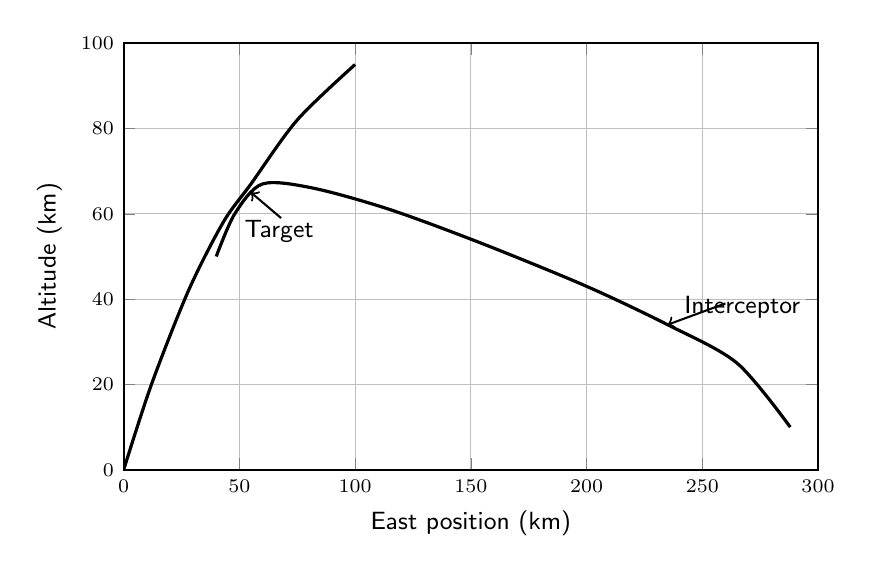
\begin{tikzpicture}
\begin{axis}[
  width=10.4cm,height=7.0cm,
  xmin=0,xmax=300,ymin=0,ymax=100,
  xtick={0,50,100,150,200,250,300},
  ytick={0,20,40,60,80,100},
  grid=major,
  axis line style={line width=0.8pt},
  tick label style={font=\scriptsize},
  label style={font=\sffamily\small},
  xlabel={East position (km)},ylabel={Altitude (km)},
]
  \addplot[line width=1.15pt,smooth] coordinates {(0,0) (12,20) (28,42) (43,58) (55,67) (75,82) (100,95)};
  \addplot[line width=1.15pt,smooth] coordinates {(40,50) (48,60) (60,67) (82,66) (115,61) (155,53) (200,43) (235,34) (265,25) (288,10)};
  \node[font=\sffamily\small,anchor=west] at (axis cs:48,56) {Target};
  \draw[->,line width=0.75pt] (axis cs:68,59)--(axis cs:55,65);
  \node[font=\sffamily\small,anchor=west] at (axis cs:238,38) {Interceptor};
  \draw[->,line width=0.75pt] (axis cs:260,39)--(axis cs:235,34);
\end{axis}
\end{tikzpicture}
}
  \caption{Altitude versus east position for an intercept trajectory.}
  \label{fig:example-air-intercept}
\end{figure}
